\section{Computer Vision und Objekterkennung}
\abschnittsautor{M. Ishak}

Die automatisierte Erfassung von Fußballspielern auf einem Spielfeld erfordert robuste Algorithmen aus dem 
Bereich der \ac{CV}. In diesem Abschnitt werden die technologischen Grundlagen der Bildverarbeitung und der 
darauf aufbauenden Objekterkennung erläutert.

\subsection{Architektur von Convolutional Neural Networks}

Ein \ac{CNN} ist eine spezielle Form von künstlichen neuronalen Netzen, die primär für die Verarbeitung von 
Bild- und Audiodaten eingesetzt wird. Im Gegensatz zu klassischen \textit{Fully Connected Networks} bewahren
\acp{CNN} die räumliche Struktur von Bilddaten und arbeiten mit einer deutlich reduzierten Anzahl an 
Parametern, was sie recheneffizienter und robuster macht~\cite{goodfellow2016deep}.

Das Kernkonzept eines \ac{CNN} ist die Faltungsschicht (Convolutional Layer). Hierbei gleiten kleine Matrizen, 
sogenannte Filter oder Kernel, schrittweise über das Eingabebild und berechnen das Skalarprodukt zwischen 
den Filtergewichten und den Bildpixeln. In den frühen Schichten des Netzwerkes lernen diese Filter einfache 
visuelle Kanten, Ecken oder Farbkontraste. In tieferen Schichten setzen sich diese einfachen Merkmale zu 
komplexeren Mustern wie spezifischen Texturen oder Objektteilen zusammen~\cite{goodfellow2016deep}. Das 
Ergebnis dieser Faltungsoperationen sind sogenannte \textit{Feature Maps} (Merkmalskarten).

Um die räumliche Auflösung der Feature Maps zu reduzieren und gleichzeitig die wichtigsten Merkmale zu 
erhalten, kommen Pooling-Schichten (z.\,B.\ Max-Pooling) zum Einsatz. Diese fassen benachbarte Pixel 
zusammen und leiten nur den dominantesten Wert weiter. Dies senkt nicht nur den Rechenaufwand signifikant, 
sondern sorgt auch für eine Translationsinvarianz~-- das Netzwerk erkennt ein gelerntes Muster unabhängig 
von dessen exakter Position im Bild.

Nach mehreren Convolutional- und Pooling-Schichten wird die resultierende mehrdimensionale Matrix 
abgeflacht (Flattening) und an eine oder mehrere \textit{Fully Connected Layers} 
(vollständig verbundene Schichten) übergeben. Diese fungieren als Klassifikator: Sie wichten die 
extrahierten, hochkomplexen Merkmale und berechnen am Ende Wahrscheinlichkeiten für die gesuchten Klassen 
(beispielsweise „Fußballspieler“, „Schiedsrichter“ oder „Ball“). Der gesamte schematische Ablauf von der 
Merkmalsextraktion bis zur Klassifikation ist in Abb.~\ref{abb:cnn-architektur} dargestellt.

\begin{figure}[htbp]
    \centering
    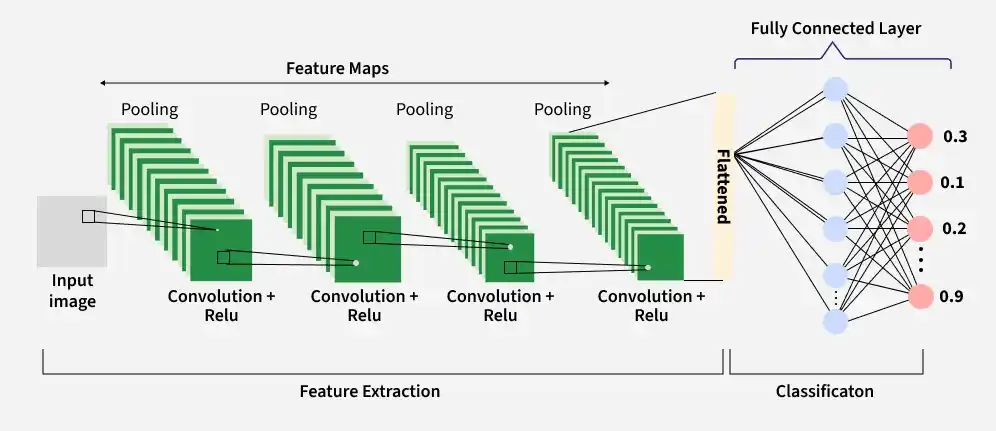
\includegraphics[width=0.9\linewidth]{images/working_of_cnn_ishak.png}
    \caption{Schematischer Aufbau eines Convolutional Neural Networks zur Bildklassifikation~\cite{gfg-cnn}.}\label{abb:cnn-architektur}
\end{figure}

\subsection{You Only Look Once (YOLO)}

Für die Objekterkennung in Echtzeit hat sich in den letzten Jahren die Modellarchitektur \ac{YOLO} als 
De-facto-Standard etabliert. Im Gegensatz zu zweistufigen Detektoren (wie etwa Faster R-CNN), die zuerst 
potenziell relevante Bildregionen vorschlagen und diese anschließend klassifizieren, formuliert \ac{YOLO} die 
Objekterkennung als ein einziges Regressionsproblem~\cite{redmon2016you}. Das gesamte Bild wird in einem 
einzigen Vorwärtsdurchlauf (Single-Pass) analysiert, um Bounding Boxes und Klassenzugehörigkeiten simultan 
vorherzusagen. Dies führt zu einer massiven Steigerung der Inferenzgeschwindigkeit.

Moderne \ac{YOLO}-Architekturen, wie das von Ultralytics entwickelte YOLOv8, bestehen grundlegend aus drei 
Hauptkomponenten: dem \textit{Backbone}, dem \textit{Neck} und dem \textit{Head}~\cite{ultralytics2023yolov8}. 
Das Backbone (basierend auf einem modifizierten CSPDarknet mit C2f-Modulen) dient als effizienter 
Feature-Extraktor. Der Neck (kombiniert aus einem Feature Pyramid Network und einem Path Aggregation Network) 
führt Merkmale aus verschiedenen Netzwerktiefen zusammen. Dies ist essenziell, um Objekte in stark 
unterschiedlichen Skalierungen zu erkennen~-- ein entscheidender Faktor im Fußball, wo Spieler in 
Kameranähe groß und auf der gegenüberliegenden Spielfeldseite sehr klein abgebildet werden. Der Head 
schlussendlich ist entkoppelt (\textit{Decoupled Head}) und arbeitet ankerfrei (\textit{Anchor-Free}): Er 
gibt auf zwei getrennten Pfaden separat die Wahrscheinlichkeiten für die Objektklassen sowie die genauen 
Koordinaten der Bounding Boxes aus.

Für die automatisierte Videoanalyse im Fußball ist YOLOv8 prädestiniert, da die hohe Inferenzgeschwindigkeit 
ein durchgehendes Frame-by-Frame-Tracking ermöglicht. Durch die Verarbeitung von hochauflösenden 
Eingabebildern (z.\,B.\ 1280 Pixel) lassen sich auch auf weite Distanzen zuverlässige Detektionen erzielen.

\subsection{Herausforderungen bei Verdeckung (Occlusion)}

Eine der größten Herausforderungen bei der optischen Verfolgung von Spielern im Fußball ist die sogenannte 
Verdeckung (Occlusion). Bei Zweikämpfen oder Standardsituationen, wie etwa einem Eckball, stehen Spieler 
dicht gedrängt und verdecken sich gegenseitig teilweise oder vollständig. Standard-Objekterkennungsmodelle 
stoßen hierbei systembedingt an ihre Grenzen.

Das Hauptproblem liegt im Post-Processing-Algorithmus der Modelle, der \ac{NMS}. \ac{YOLO} generiert für 
dasselbe Objekt oft mehrere leicht verschobene Bounding Boxes. Um diese zu bereinigen, berechnet die 
\ac{NMS} den \ac{IoU}-Wert~-- das Verhältnis der Schnittfläche zur Vereinigungsfläche zweier 
Boxen $A$ und $B$:
\begin{equation}
    \text{IoU}(A, B) = \frac{|A \cap B|}{|A \cup B|}
\end{equation}
Überschreitet dieser Wert einen definierten Schwellenwert (z.\,B.\ $0{,}45$), geht der Algorithmus davon aus, 
dass beide Boxen dasselbe Objekt markieren, und löscht die Box mit der geringeren \textit{Confidence} 
(Konfidenz)~\cite{bodla2017soft}. Stehen jedoch zwei Fußballspieler im Zweikampf dicht hintereinander, 
überschneiden sich ihre echten Bounding Boxes extrem stark. Standard-\ac{NMS} bewertet den teilweise 
verdeckten Spieler fälschlicherweise als redundante Detektion des vorderen Spielers und unterdrückt 
ihn komplett.

Um diese Problematik zu beheben, erfordert es spezialisierte Lösungsansätze. Einerseits muss durch gezieltes 
Fine-Tuning auf fußballspezifische Datensätze trainiert werden, die eine hohe Dichte an Spielerverdeckungen 
(Ground Truth) aufweisen, wie in Abb.~\ref{abb:occlusion-beispiel} exemplarisch dargestellt ist. 
Andererseits kommen spezifische Data-Augmentation-Methoden sowie angepasste \ac{IoU}-Schwellenwerte 
oder tolerantere Verfahren wie Soft-\ac{NMS}~\cite{bodla2017soft} zum Einsatz, um die Detektionsrate 
(Recall) bei starker Verdeckung signifikant zu steigern.

\begin{figure}[htbp]
    \centering
    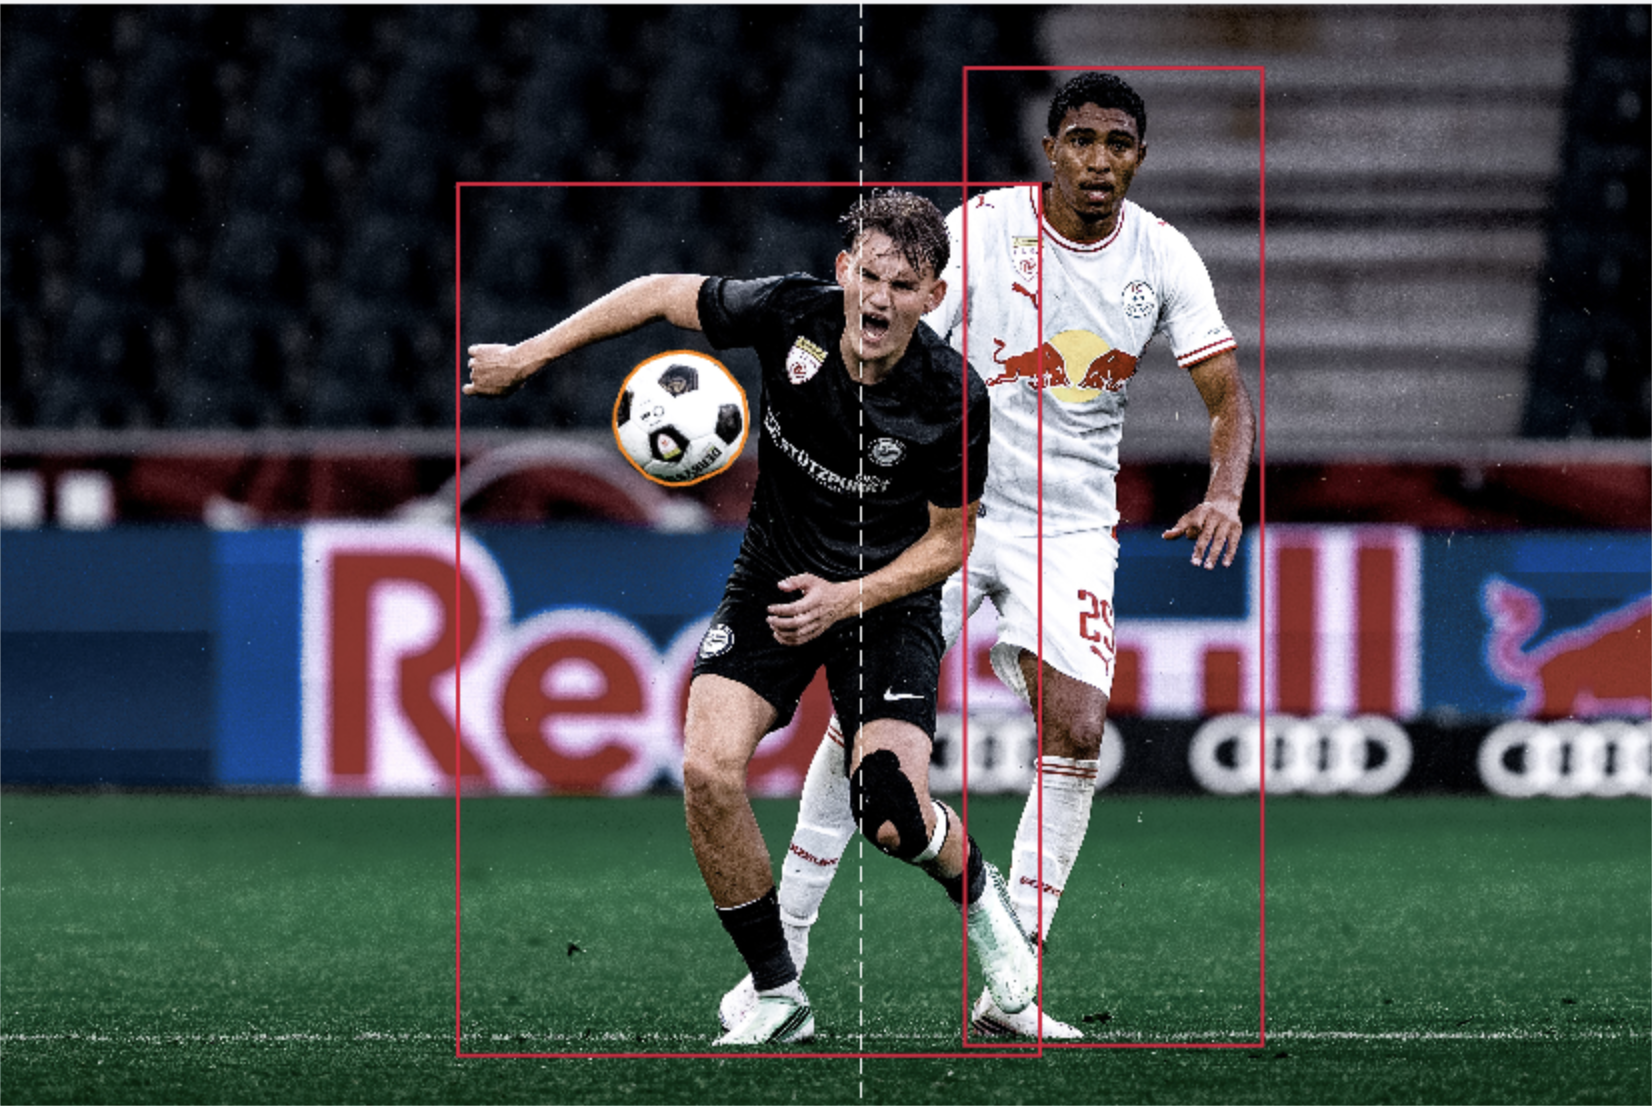
\includegraphics[width=0.75\linewidth]{images/roboflow_bounding_box_ishak.png}
    \caption{Beispiel einer starken Verdeckung (Occlusion) im Fußball. Der hintere Spieler wird trotz massiver Überlappung separat annotiert und detektiert (eigene Darstellung in Roboflow).}\label{abb:occlusion-beispiel}
\end{figure}

\subsection{Transfer Learning und Fine-Tuning}

Das Training eines tiefen neuronalen Netzes von Grund auf (Training from Scratch) erfordert 
hunderttausende annotierte Bilder sowie massive Rechenkapazitäten, um grundlegende Merkmale wie Kanten 
und einfache geometrische Formen zu erlernen. Um diese Ressourcenhürde zu umgehen, wird in der modernen 
Bildverarbeitung das Prinzip des \textit{Transfer Learning} (Wissenstransfer) angewandt~\cite{pan2009survey}.

Dabei wird ein Basismodell verwendet, das bereits auf einem enormen, generischen Datensatz~-- wie 
dem \ac{COCO}-Datensatz mit über 330.000 Bildern und 80 Objektklassen~-- vortrainiert wurde. Die 
unteren Schichten (Backbone) dieses Modells haben bereits die Fähigkeit zur generellen Merkmalsextraktion 
perfektioniert. Beim sogenannten \textit{Fine-Tuning} werden die Gewichte des Netzes mit einer reduzierten 
Lernrate auf einen neuen, spezifischen Zieldatensatz~-- in diesem Fall fußballspezifische Aufnahmen~-- 
nachtrainiert und angepasst. Dies ermöglicht es, das Modell mit einer verhältnismäßig kleinen Menge an 
domänenspezifischen Trainingsdaten (wenige tausend Bilder) hocheffizient auf die Zielklassen 
(Spieler, Tormann, Ball, Schiedsrichter) zu spezialisieren, während irrelevante Klassen des 
Ursprungsmodells verworfen werden.

\subsection{Evaluierungsmetriken der Objekterkennung}

Um die Leistungsfähigkeit und Genauigkeit eines Objekterkennungsmodells objektiv beurteilen zu können, 
werden standardisierte Metriken herangezogen~\cite{padilla2020survey}. Grundlage hierfür ist der 
bereits erwähnte \ac{IoU}-Wert. Ein Detektionsergebnis gilt als \textit{True Positive} (TP), wenn der 
\ac{IoU} zwischen der vorhergesagten Bounding Box und der tatsächlichen Ground-Truth-Box einen 
definierten Schwellenwert (meist $0{,}50$) überschreitet. Liegt der Wert darunter oder wird ein 
Hintergrundobjekt fälschlicherweise markiert, resultiert ein \textit{False Positive} (FP). Wird ein 
reales Objekt vom Modell komplett übersehen, spricht man von einem \textit{False Negative} (FN).

Aus diesen Klassifikationen leiten sich die zwei fundamentalen Metriken ab:
\begin{itemize}
    \item \textbf{Precision (Genauigkeit):} Berechnet sich aus $\frac{TP}{TP + FP}$. Sie gibt an, wie viel Prozent der vom Modell gesetzten Bounding Boxes tatsächlich korrekte Objekte einkreisen. Eine hohe Precision bedeutet wenige Fehlalarme (z.\,B.\ wenn Werbebanden fälschlicherweise als Spieler erkannt werden).
    \item \textbf{Recall (Trefferquote):} Berechnet sich aus $\frac{TP}{TP + FN}$. Sie gibt an, wie viel Prozent der tatsächlich auf dem Bild vorhandenen Objekte vom Modell gefunden wurden. Im Kontext der Spielerverdeckung (Occlusion) ist der Recall die kritischste Metrik, da er aufzeigt, wie viele verdeckte Spieler fälschlicherweise übersehen wurden.
\end{itemize}

Um das Modell über verschiedene Konfidenz-Schwellenwerte hinweg bewerten zu können, wird die Fläche unter 
der Precision-Recall-Kurve berechnet, die sogenannte \textit{Average Precision} (AP). Der Mittelwert der 
AP über alle trainierten Klassen hinweg ergibt die \textit{mean Average Precision} (mAP). In aktuellen 
Evaluierungen wird häufig die Metrik \textbf{mAP@50--95} herangezogen. Hierbei wird die mAP über zehn 
verschiedene \ac{IoU}-Schwellenwerte (von $0{,}50$ bis $0{,}95$ in $0{,}05$-Schritten) 
gemittelt~\cite{padilla2020survey}. Ein hoher mAP@50--95-Wert garantiert nicht nur, dass das Objekt 
überhaupt gefunden wurde, sondern dass die Kanten der Bounding Box millimetergenau am Objekt anliegen~-- eine 
essenzielle Voraussetzung für die anschließende geometrische Homografie-Transformation in 
2D-Spielfeldkoordinaten.

\subsection{Verlustfunktionen (Loss-Architektur) in YOLOv8}

Während des Trainingsprozesses optimiert YOLOv8 seine Netzwerkgewichte durch die Minimierung einer 
zusammengesetzten Verlustfunktion (Loss Function). Da der Decoupled Head von YOLOv8 Klassifikation und 
Lokalisierung trennt, setzt sich der Gesamtverlust aus drei gewichteten Komponenten 
zusammen~\cite{ultralytics2023yolov8}:
\begin{equation}
    \mathcal{L}_{\text{total}} = \lambda_{\text{box}} \mathcal{L}_{\text{CIoU}} + \lambda_{\text{dfl}} \mathcal{L}_{\text{DFL}} + \lambda_{\text{cls}} \mathcal{L}_{\text{BCE}}
\end{equation}

Für die Klassifikation der vier Zielklassen kommt der \ac{BCE}-Verlust $\mathcal{L}_{\text{BCE}}$ zum Einsatz, 
der für jede Klasse unabhängig die Wahrscheinlichkeit berechnet. Für die räumliche Präzision der Bounding 
Boxes~-- welche für die Berechnung des Spieler-Fußpunktes entscheidend ist~-- kombiniert YOLOv8 zwei 
spezialisierte Lokalisierungsverluste:
\begin{itemize}
    \item \textbf{Complete IoU Loss ($\mathcal{L}_{\text{CIoU}}$):} Im Gegensatz zum einfachen \ac{IoU}-Verlust berücksichtigt der \ac{CIoU} zusätzlich den euklidischen Abstand zwischen den Mittelpunkten der vorhergesagten Box $b$ und der Ground-Truth-Box $b^{gt}$ sowie die Konsistenz des Seitenverhältnisses (Aspect Ratio) $v$~\cite{zheng2020distance}:
    \begin{equation}
        \mathcal{L}_{\text{CIoU}} = 1 - \text{IoU} + \frac{\rho^2(b, b^{gt})}{c^2} + \alpha v
    \end{equation}
    Hierbei bezeichnet $c$ die Diagonale des kleinsten umschließenden Rechtecks beider Boxen. Dadurch konvergiert das Modell deutlich schneller auf die exakte Körperform von stehenden oder laufenden Spielern.
    \item \textbf{Distribution Focal Loss ($\mathcal{L}_{\text{DFL}}$):} Bei starker Verdeckung (Occlusion) im Strafraum sind die Kanten einer Bounding Box oft mehrdeutig, da Körperteile durch Gegenspieler verdeckt werden. Anstatt die Box-Koordinaten als starre Einzelwerte (Dirac-Delta-Verteilung) vorherzusagen, modelliert der \ac{DFL} die Position jeder Box-Kante als diskrete Wahrscheinlichkeitsverteilung~\cite{li2020generalized}. Dies erlaubt es dem Netzwerk, Unsicherheiten an verdeckten Körperkanten mathematisch abzubilden und dennoch scharfe Begrenzungsboxen zu schätzen.
\end{itemize}

\subsection{Mathematische Grundlagen der Data Augmentation}

Um eine Überanpassung (Overfitting) des Modells an die Trainingsdaten zu verhindern und die 
Generalisierungsfähigkeit bei schwierigen Licht- und Verdeckungsverhältnissen zu erhöhen, wird 
während des Fine-Tunings eine dynamische Datenaugmentierung (Online Data Augmentation) durchgeführt. 
Die Trainingsbilder werden dabei in jeder Epoche vor dem Durchlauf durch das Netz zufällig transformiert. 
Tab.~\ref{tab:augmentation-methoden} fasst die für die Fußballanalyse relevanten Augmentierungsverfahren 
und deren spezifischen Nutzen zusammen.

\begin{table}[htbp]
    \centering
    \caption{Eingesetzte Data-Augmentation-Verfahren zur Steigerung der Modellrobustheit}\label{tab:augmentation-methoden}
    \begin{tabularx}{\linewidth}{llX}
        \tabkopf{}
        Verfahren & Operation & Nutzen im Fußball-Kontext \\
        Mosaic~\cite{bochkovskiy2020yolov4} & 4-Bild-Collage & Erkennung kleiner Spieler \& Kontextvarianz \\
        Random Erasing~\cite{zhong2020random} & Pixelmaskierung & Simulation teilweiser Spielerverdeckung \\
        MixUp & Bildüberblendung & Robustheit bei direktem Zweikampf-Kontakt \\
        HSV-Shift & Farbraumanpassung & Unabhängigkeit von Licht, Schatten \& Trikots \\
        Horizontal Flip & Achsenspiegelung & Richtungsunabhängige Lauferkennung \\
    \end{tabularx}
\end{table}

Besonders hervorzuheben sind hierbei die Verfahren \textit{Mosaic}~\cite{bochkovskiy2020yolov4} und 
\textit{Random Erasing}~\cite{zhong2020random}. Bei der Mosaic-Augmentierung werden vier unterschiedliche 
Trainingsbilder skaliert und zu einem einzigen Trainingsframe zusammengesetzt. Dadurch sieht das Modell 
in einem einzigen Batch unterschiedliche Stadionperspektiven und Objektskalierungen gleichzeitig. Durch 
Random Erasing werden gezielt Bildbereiche innerhalb der Bounding Boxes gelöscht, wodurch das \ac{CNN} 
gezwungen wird, seine Aktivierung nicht allein auf die vollständige Spielersilhouette zu stützen, sondern 
auch Teilmerkmale wie Kopf, Schultern oder Stutzen als hinreichende Indikatoren für eine Detektion zu 
gewichten.